\documentclass[10pt,letterpaper]{article}
\usepackage{url}
\usepackage[colorlinks,urlcolor=blue]{hyperref}
\usepackage[UTF8]{inputenc}
%\usepackage[latin1]{inputenc}
\usepackage[T1]{fontenc}
\usepackage{uarial}
\renewcommand\familydefault{\sfdefault}
\usepackage{amsmath,amssymb,amsfonts,latexsym,cancel, wrapfig, multicol,enumerate,graphicx, xcolor,paralist,tikz,tkz-tab,dsfont}
\usepackage[letterpaper,showframe=false]{geometry}
\usepackage[spanish]{babel}
\usepackage{color}
\usepackage{hyperref}
%colores------------------------------------------------
\definecolor{encabezado}{RGB}{64,107,204} % % % Principal
\definecolor{titulos}{RGB}{112,90,45}
\definecolor{actividades}{RGB}{112,90,45}
\definecolor{cuadro1}{RGB}{204,219,226}
\definecolor{cuadro2}{RGB}{226,210,178} % % % tercero
\definecolor{cuadro3}{RGB}{255,230,179}
\definecolor{CRecapitulacion}{RGB}{204,219,226}
\definecolor{CcontenidosObjetivos}{RGB}{204,219,226} % % Secundario
\definecolor{ContenidosObjetivos}{RGB}{112,90,45}
\definecolor{numerosTabla}{RGB}{0,0,0}


%--------------- Colores IS22-----------------------
%\definecolor{encabezado}{RGB}{0,134,75} % % % Principal
%\definecolor{titulos}{RGB}{1,110,111}
%\definecolor{actividades}{RGB}{1,110,111}
%\definecolor{cuadro1}{RGB}{173,211,144}
%\definecolor{cuadro2}{RGB}{249,241,133} % % % tercero
%\definecolor{cuadro3}{RGB}{253,199,117}
%\definecolor{CRecapitulacion}{RGB}{188,228,230}
%\definecolor{CcontenidosObjetivos}{RGB}{188,228,230} % % Secundario
%\definecolor{ContenidosObjetivos}{RGB}{1,110,111}
%\definecolor{numerosTabla}{RGB}{70,70,70}

%--------------- Colores antes de IS22-----------------------
%\definecolor{encabezado}{RGB}{65,130,185}
%\definecolor{titulos}{RGB}{65,130,185}
%\definecolor{actividades}{RGB}{239,80,0}
%\definecolor{cuadro1}{RGB}{216,216,216}
%\definecolor{cuadro2}{RGB}{249,206,17}
%\definecolor{cuadro3}{RGB}{239,159,77}
%\definecolor{CRecapitulacion}{RGB}{216,216,216}
%\definecolor{CcontenidosObjetivos}{RGB}{138,186,212}
%\definecolor{ContenidosObjetivos}{RGB}{86,86,86}
%\definecolor{numerosTabla}{RGB}{48,103,133}
%-------------------------------------------------------

\DeclareGraphicsExtensions {.pdf,.png,.jpg}

%Dimensiones-------------------------------------------
\textheight=26cm
\textwidth=20 cm
\topmargin=-3.2 cm
\oddsidemargin=-2 cm
\evensidemargin=0 cm
\parskip=0 mm
\parindent=0 mm
%-----------------------------------------------------


%\usepackage[T1]{fontenc}
\usepackage{uarial}
\renewcommand\familydefault{\sfdefault}
%\usepackage{blindtext}

\newcommand{\URLLibroMN}{\href{https://ezproxy.itcr.ac.cr/login?url=https://www.bibliotecaebook.com/my-library}{\textbf{Acceso al e-book}} Libro de Métodos Numéricos. Autor Jeffry Chavarría Molina.}

\newcommand{\CursoOctave}{\href{https://lugfi.github.io/curso-octave/index.html}{\textbf{Ingreso al curso}}}

\newcommand{\PaqueteSymbolic}{\href{https://docs.sympy.org/latest/tutorials/intro-tutorial/index.html}{\textbf{Paquete Sympy:}} Paquete para realizar cálculo simbólico en Python}
%--------------------------------
%Videos


\newcommand{\URLVideoUno}{\href{https://youtu.be/_7Aw-ay67DM}{\textbf{Vídeo 1:}} Integración con datos no igualmente espaciado}

\newcommand{\URLVideoDos}{\href{https://tecnube1-my.sharepoint.com/:v:/g/personal/ccalderon_itcr_ac_cr/EfR-z83flapBtUcMU36DMr4BlEX-YLvYJBM7eMtV8kM4Mw?e=9Ed7WD}{\textbf{Video 2:}} Cuadratura Gaussiana. Introducción}

\newcommand{\URLVideoTres}{\href{https://tecnube1-my.sharepoint.com/:v:/g/personal/ccalderon_itcr_ac_cr/EZJCmoE_ZydJqdjObEAX0EcBSlz-IyN2drdlT4QuWE759g?e=3r3SLz}{\textbf{Video 3:}} Cuadratura Gaussiana. Ejemplo}

\newcommand{\URLVideoCuatro}{\href{https://tecnube1-my.sharepoint.com/:v:/g/personal/ccalderon_itcr_ac_cr/ETdNUpQs4Q5LjHNWW62PxP8BUNPz02wIHSAs_nfhxJRW2g?e=5s6yyh}{\textbf{Video 4:}} Gauss-Legendre}

\newcommand{\URLVideoCinco}{\href{https://youtu.be/j0SyekJzuvg}{\textbf{Video 5:}} Cuadratura Gaussinaa en Octave}


%------------Vídeos teoricos---------------
\newcommand{\URLVideoTeoriaActiI}{\href{https://drive.google.com/file/d/1Is-lhFgiC0lT138Ikfc-pgqc2trrvBBq/view?usp=sharing}{\textbf{Vídeo de teoría 1:}}  Complementario al libro}
\newcommand{\URLVideoTeoriaActiII}{\href{https://drive.google.com/file/d/1kloExvEhsScDhAK6WMXRjhp5rQ62zYDm/view?usp=sharing}{\textbf{Vídeo de teoría 2:}} Complementario al libro}
\newcommand{\URLVideoTeoriaActiIII}{\href{https://drive.google.com/file/d/1H7o1l6RkJaNmG_7-_cLjfnSolojOus38/view?usp=sharing}{\textbf{Vídeo de teoría 3:}} Complementario al libro}


%---------Infografías-----------------



%----------Solucionario-------------
\newcommand{\FolletoPractica}{\href{https://tecnube1-my.sharepoint.com/:b:/g/personal/jchavarria_itcr_ac_cr/ESbC_k0vPWdMovfv0-d9GpoBcM31nPWa26ScY419frpBdw?e=hutomi}{\textbf{Folleto de práctica}} Folleto completo de práctica del curso.}

\newcommand{\FolletoPracticaDOS}{\href{https://tecnube1-my.sharepoint.com/:b:/g/personal/jchavarria_itcr_ac_cr/ESbC_k0vPWdMovfv0-d9GpoBcM31nPWa26ScY419frpBdw?e=hutomi}{\textbf{Folleto de práctica}}}


%----------Podcast---------------------------------------------

\newcommand{\URLpodcast}{\href{https://soundcloud.com/angie-solis-palma/logica-matematica-y-conectivas-logicas?utm_source=clipboard\&utm_campaign=wtshare\&utm_medium=widget\&utm_content=https\%253A\%252F\%252Fsoundcloud.com\%252Fangie-252Fsol-palmamama}{\textbf{Podcast:}} Lógica matemática.}



\newcommand{\URLFacebook}{\href{https://tecdigital.tec.ac.cr/dotlrn/catedras.tec/matematicadiscreta/one-community?page_num=0&loc=}{enlace}}

\newcommand{\URLPortalComunidad}{\href{https://tecdigital.tec.ac.cr/dotlrn/catedras.tec/matematicadiscreta/one-community?page_num=0&loc=}{portal de la comunidad del TecDigital para MD}}

\newcommand{\URLPortalGrupoTecDigital}{\href{https://tecdigital.tec.ac.cr/dotlrn/classes/MA/MA1403/S-2-2022.CA.MA1403.6/one-community?page_num=0&loc=}{portal del TecDigital para el grupo 06}}

\newcommand{\URLConsulta}{\href{https://tecdigital.tec.ac.cr/dotlrn/catedras.tec/matematicadiscreta/one-community?page_num=5&loc=}{enlace}}

\newcommand{\ImagenDM}{
\includegraphics[scale=0.7]{imagenes/MN.png}}

\newcommand{\Motivacion}{
\includegraphics[scale=0.6]{imagenes/motivacion.png}}


\begin{document}
\setlength{\parskip}{0.3cm}

%Encabezado-----------------------------------------------------------------------------------	






\begin{center}
{ \fboxsep 12pt
	\fcolorbox {encabezado}{encabezado}{
	\begin{minipage}[t]{19.5cm}
		{\color{white} 
		TEC | MÉTODOS NUMÉRICOS GRUPO SEMIPRESENCIAL \hfill  II SEMESTRE 2026
 \\
		\rule[0.1cm]{19.5cm}{0.01cm}
		\begin{center}
			{\Huge  \textbf{Semana 12}}
		\end{center}
		\vspace{-0.5cm}
		\rule[0cm]{19.5cm}{0.01cm}
		\begin{center}
			{  \textbf{Integración Numérica}}
		\end{center}
					}
	\vspace{-0.5cm}
	\end{minipage}
	} 
}
\end{center}


%Pagina1-------------------------------------------------------------------------
\begin{minipage}[c]{14cm}
	\begin{center}
		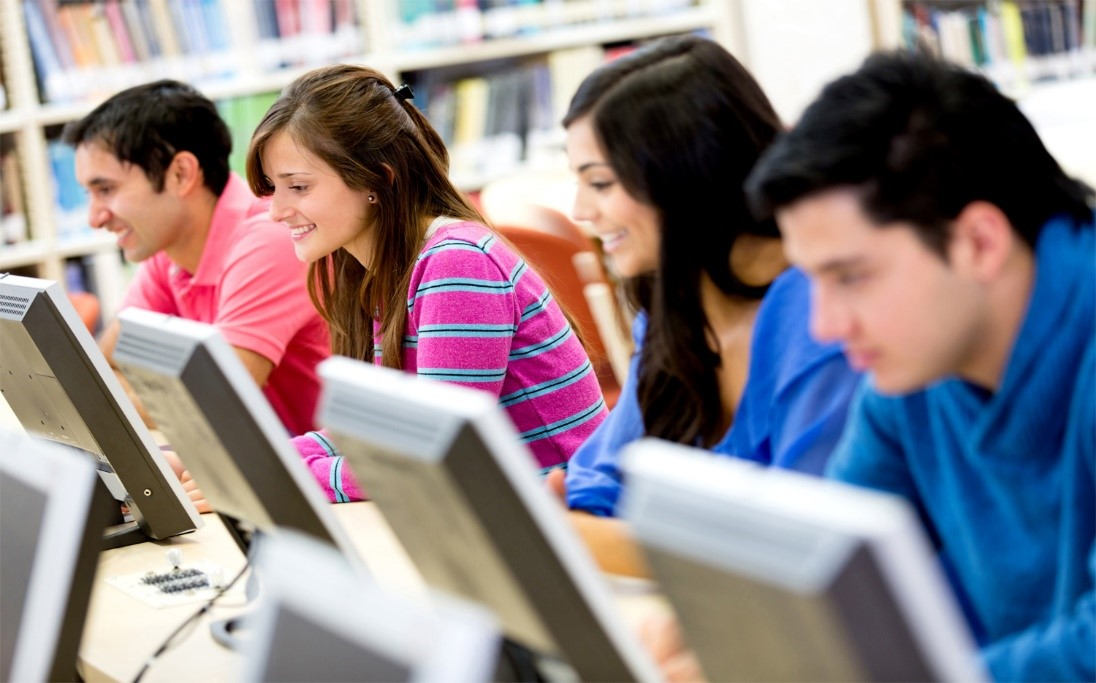
\includegraphics[height=5.4cm,width=11cm]{imagenes/estudiantes}
	\end{center}
		
{\color{titulos} {\large \textbf{Descripción para la semana:}}}\\
		
La clase de la \textbf{semana 12 será asincrónica}. Trabajarán en la página web \href{https://jchavarriam-pixel.github.io/ITCR_CURSOS/MN/IntegracionNumerica/}{\textbf{Integración numérica · Métodos Numéricos}} los contenidos de esta semana: trapecio, Simpson y cuadratura gaussiana. Sigan el orden de las secciones: \textbf{vean primero cada video}, intenten los cálculos y luego consulten el desarrollo escrito para comparar fórmulas, procedimientos y resultados. La regla del rectángulo y su versión compuesta ya fueron estudiadas.

{\color{titulos} {\large \textbf{ Modo de trabajo:}}}
		
{ \fboxsep 12pt
	\fcolorbox {cuadro1}{cuadro1}{
		\begin{minipage}[l][9.6cm]{3.15cm}
			\begin{center}
				
\includegraphics[scale=0.2]{imagenes/uno}
			\end{center}
			{\color{ContenidosObjetivos} {\large Material a utilizar}} \\ \\
			{\footnotesize
\href{https://jchavarriam-pixel.github.io/ITCR_CURSOS/MN/IntegracionNumerica/}{\textbf{Guía web de integración numérica}}\\[0.2cm]
Videos, explicaciones escritas, fórmulas, cálculos y resultados.\\[0.2cm]
Consulten también las notas de clase enlazadas en la página.
} 
\vspace{0.5cm}
						
		\end{minipage}
		}
}
{ \fboxsep 12pt
		\fcolorbox {cuadro2}{cuadro2}{
			\begin{minipage}[l][9.6cm]{3.9cm}
				\begin{center}
					
\includegraphics[scale=0.2]{imagenes/dos}
				\end{center}
				{\color{ContenidosObjetivos} {\large Vídeos}} \\ \\
				{\footnotesize
\textbf{Orden de estudio:}\\[0.2cm]
\textbf{02--05:} Trapecio y trapecio compuesto.\\[0.2cm]
\textbf{06--10:} Simpson, error y Simpson compuesto.\\[0.2cm]
\textbf{11--15:} Cuadratura gaussiana y Gauss-Legendre.\\[0.2cm]
En cada sección, vean primero el video y hagan pausas para resolver por su cuenta.
}
\end{minipage}
	}
}
{ \fboxsep 12pt
	\fcolorbox {cuadro3}{cuadro3}{
		\begin{minipage}[l][9.6cm]{3.15cm}
			\begin{center}
				
\includegraphics[scale=0.2]{imagenes/tres}
			\end{center}
			{\color{ContenidosObjetivos} {\large Evaluación}} \\ \\
			 \footnotesize 
			 \textbf{Semana 13:}

La clase será \textbf{presencial} y se realizarán \textbf{quices sobre interpolación y regresión}.

Repasen las notas, los procedimientos y los ejercicios trabajados en ambos temas.
\vfill
\end{minipage}
	} 
} 
\end{minipage}\hspace{0.2cm}\begin{minipage}[c]{5cm}
\begin{center}
{ \fboxsep 12pt
		\fcolorbox {CcontenidosObjetivos}{CcontenidosObjetivos}{
\begin{minipage}[l][21cm]{5cm}
\begin{center}
	\ImagenDM
\end{center}
					
{\color{ContenidosObjetivos}\textbf{ \small Contenidos:}}\\
					
{\footnotesize
{ \tiny $\blacksquare$} Métodos numéricos para la integración de funciones \\ \\
{ \tiny $\blacksquare$}  Programación de métodos para la integración de funciones\\\\[0.2cm]
{ \tiny $\blacksquare$} Cuadratura Gaussiana\\ \\
{ \tiny $\blacksquare$} Métodos de Cuadratura Gauss-Legendre\\
}

{\color{white}\rule[0.1cm]{5cm}{0.01cm}}
		{\color{ContenidosObjetivos} \textbf{ \small Objetivos:}}\\
					
{\footnotesize
{ \tiny $\blacksquare$} Estudiar métodos asociados la integración de funciones \\ \\
{ \tiny $\blacksquare$} Programar los métodos para
la integración de funciones\\[0.2cm]
{ \tiny $\blacksquare$} Estudiar los métodos de Cuadratura Gaussiana para aproximar integrales. \\ \\
{ \tiny $\blacksquare$} Programar los métodos de Gauss-Legendre.
}

{\color{white}\rule[0.1cm]{5cm}{0.01cm}}\\

%\vspace{2cm}
%\hspace{-7pt}\begin{minipage}[4cm]{5cm}
%\begin{center}
%
\includegraphics[scale=0.14]{imagenes/QRFacebook}
%
%Comunidad de la cátedra de Matemática Discreta en el tecDigital (\URLFacebook).
%\end{center}
%\end{minipage}

\end{minipage}
}}
\end{center}
\end{minipage}	 
%----------------------------------------------------------------------------


\newpage

%Página2----------------------------------------------------------------------
\begin{multicols}{2}
Organicen el estudio por etapas. Los videos y las explicaciones escritas se complementan: los primeros muestran el proceso paso a paso y el texto permite repasar las fórmulas, los cálculos y los resultados.

{\color{actividades}\textbf{Actividad 1: Trapecio (videos 02--05)}}
\begin{itemize}
\item Estudien la deducción y el ejemplo de la regla del trapecio; luego, su versión compuesta.
\item Reproduzcan las aproximaciones de la integral de $\operatorname{sen}(x)/x$ en $[1,2]$ con uno y con tres trapecios.
\item Comparen el error real con la cota teórica. Identifiquen el papel de $h$, de $n$ y de la segunda derivada.
\end{itemize}

{\color{actividades}\textbf{Actividad 2: Simpson (videos 06--10)}}
\begin{itemize}
\item Estudien la deducción de la regla de Simpson, su ejemplo y el análisis del error.
\item Continúen con la deducción y el ejemplo de Simpson compuesto. Identifiquen la condición de que $n$ sea par y el patrón de los coeficientes.
\item Repitan los cálculos antes de consultar la solución. Distingan el error real de su cota y reconozcan el uso de la cuarta derivada.
\end{itemize}

\columnbreak
{\color{actividades}\textbf{Actividad 3: Cuadratura gaussiana (videos 11--15)}}
\begin{itemize}
\item Revisen el planteamiento de la cuadratura gaussiana y la elección de nodos y pesos.
\item Estudien Gauss-Legendre de dos puntos: deducción y ejemplos. Continúen con la deducción y el ejemplo de tres puntos.
\item Practiquen el cambio de variable de $[a,b]$ a $[-1,1]$, incluyendo el factor que multiplica la integral.
\item Revisen el resumen de dos, tres y cuatro puntos; identifiquen los nodos, pesos y grados de exactitud correspondientes.
\end{itemize}

{\color{actividades}\textbf{Actividad 4: Síntesis y preparación}}
\begin{itemize}
\item Elaboren un cuadro con cada regla, sus condiciones de aplicación y la información necesaria para estimar el error, cuando el material la incluya.
\item Comparen las aproximaciones de los ejemplos y registren las dudas que surjan.
\item Repasen interpolación y regresión para los quices presenciales de la semana 13.
\end{itemize}
El video 01, sobre rectángulo compuesto, queda como repaso opcional de lo ya estudiado.
\end{multicols}

\newpage
{\color{titulos}\Large\textbf{Ejercicios asignados para la semana 12}}

Realicen los siguientes ejercicios como parte del trabajo de la semana 12. Los correspondientes a la regla del rectángulo sirven como repaso de lo ya estudiado.

\begin{multicols}{2}
{\color{actividades}\textbf{Libro de texto}}
\begin{itemize}
\item Página 350, lista de ejercicios 5.3: ejercicios \textbf{2, 3a, 3b, 4 y 5}.
\item Página 356, lista de ejercicios 5.4: ejercicios \textbf{1, 2b y 3b}.
\item Página 360, lista de ejercicios 5.5: ejercicios \textbf{1, 2 y 3}.
\item Página 371, lista de ejercicios 5.6: \textbf{todos los ejercicios}.
\end{itemize}

\columnbreak
{\color{actividades}\textbf{Folleto de prácticas}}
\begin{itemize}
\item Página 78: ejercicio \textbf{6.2.7 (partes 1, 3, 4 y 5)}.
\item Página 79: ejercicio \textbf{6.2.10 (partes 3, 4 y 5)}.
\item Página 80: ejercicio \textbf{6.2.16 (partes 1 y 2)}.
\item Página 83: ejercicio \textbf{6.2.21 (parte 2)}.
\item Página 84: ejercicio \textbf{6.2.22 (partes 1 y 2)}.
\item Página 85: ejercicio \textbf{6.2.23 (parte 1)}.
\end{itemize}
\end{multicols}



{ \fboxsep 12pt
\fcolorbox {CRecapitulacion}{CRecapitulacion}{
\begin{minipage}[c]{12cm}
{\color{ContenidosObjetivos}\large {\large Recapitulación}:}\\
		
Se les recuerda la importancia de completar las actividades asignadas de la sección virtual para un desarrollo adecuado de su aprendizaje. Completen el recorrido de estudio de esta semana asincrónica y conserven sus cálculos para repasarlos y consultar sus dudas. \\
		
Se le recuerda que no está solo en el proceso. Puede realizar sus dudas en el grupo de Teams.\\
		

\end{minipage}
		\begin{minipage}[c]{7cm}
			\begin{center}
				\Motivacion
			\end{center}
			
		\end{minipage}
	}
}

%{\color{actividades} \textbf{   $\bullet$ Códigos QR de los vídeos:}}\\
%\begin{center}
%\begin{tabular}{|c|c|c|c|}
%\hline 
%\textbf{¿Para que sirven las matemáticas?} & \textbf{Motivación a la lógica} & \textbf{Vídeo de teoría 1} &\textbf{Vídeo de teoría 2} \\ \hline &&&\\  
%
\includegraphics[scale=0.1]{imagenes/QRMoti1} & 
\includegraphics[scale=0.1]{imagenes/QRMoti2} & 
\includegraphics[scale=0.1]{imagenes/QRVideo1} & 
\includegraphics[scale=0.1]{imagenes/QRVideo2}\\ 
%\hline 
%\textbf{Vídeo 3}&\textbf{Vídeo 4}&\textbf{Vídeo 5}&\\ 
%\hline &&&\\  
% 
\includegraphics[scale=0.1]{imagenes/QRVideo3} & 
\includegraphics[scale=0.1]{imagenes/QRVideo4} & 
\includegraphics[scale=0.1]{imagenes/QRVideo5} & \\ \hline
%\end{tabular} 
%\end{center}
\end{document}